Nachdem die grundlegende Herangehensweise der Technik geklärt wurde, wird in diesem Kapitel auf Design- und Konzeptionsideen eingegangen, die bis zur finalen Umsetzung aufkamen. Die meisten der verschiedenen Umsetzungsmöglichkeiten wurden bei der Entwicklung getestet und ihre Praktikabilität analysiert, woraus sich das im letzten Unterpunkt beschriebene, finale Interaktionsdesign für eine mögliche Studie abgeleitet wurde.

\section{Module}
Die Technik besteht aus den folgenden vier Grundbausteinen: Der World in Miniature, der miniaturisierten Nutzerplattform in der WIM, einem Selektionstool und dem Portalfenster.

\textbf{WIM:}\\
Die verwendete WIM soll in unserem Fall eine exakte Kopie der Umgebung sein und nicht wie bei Pierce et al. aus einer vereinfachten Version bestehen. Die Nutzer sollen in der Lage sein, auch feinere Details in der WIM erkennen zu können. 

 \textbf{Selektionstool:}\\
Um die Technik nutzen zu können bedarf es eines Werkzeugs, mit welchem der Nutzer mit der WIM interagieren kann. 

\textbf{Minaturisierte Nutzerplattform:}\\
\begin{figure}[h!]
  \centering
  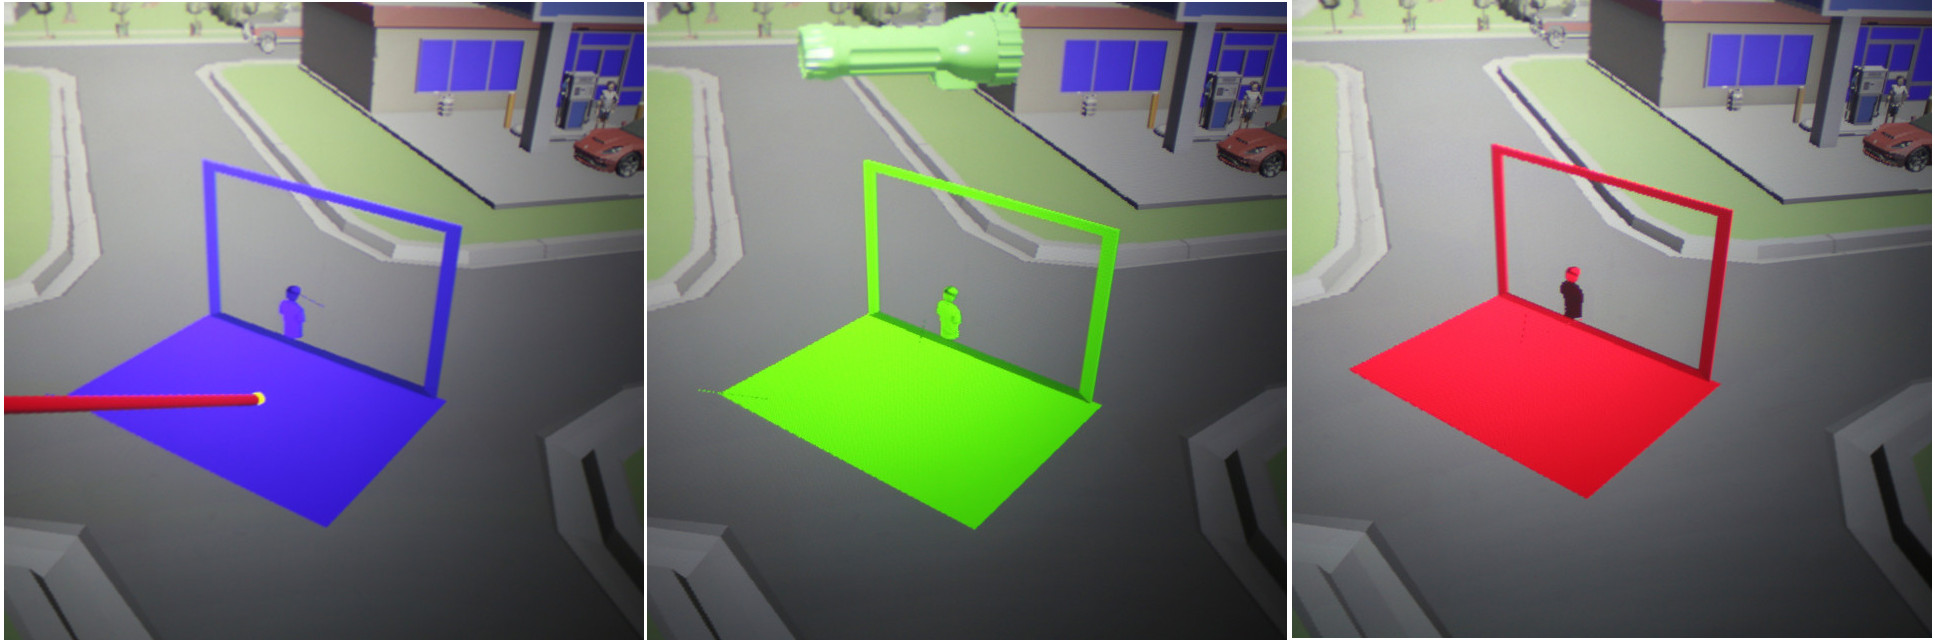
\includegraphics[width=0.8\textwidth]{images/platform_bgr.jpg}
  \caption{Die drei Versionen der Nutzerplattform in der WIM: Die Blaue dient zur Planung der Position in der WIM. Wird diese bestätigt wird eine grüne Kopie erstellt. Nach dem Teleport zeigt die rote Plattform den tatsächlichen, aktuellen Aufenthaltsort der Nutzer in der Umgebung an}
  \label{fig:todo}
\end{figure}
Die miniaturisierte Nutzerplattform (im Folgenden: Plattform) repräsentiert die Nutzer (in Form von Avataren), die 3D-Leinwand sowie die Bodenplatte, welche den getrackten Bereich des realen Raumes darstellt. Diese Plattform ist in der WIM zum Beispiel an der Stelle (in rot, vgl. Abbildung 8.1) sichtbar, an denen sich die Nutzer zu diesem Zeitpunkt befinden, damit sie ihre aktuelle Position in der Umgebung einschätzen können. Dabei ist es wichtig, dass die Tracking-Koordinaten, welche die Positionen der Köpfe der Nutzer bestimmen in dieser Version aktualisiert werden, damit die Avatarpositionen denen der Nutzer im realen Raum entsprechen. Eine zweite Form dieser Repräsentation soll nämlich auch zur Reiseplanung dienen. Indem diese Plattform vom steuernden Nutzer in der WIM platziert wird, spezifiziert er die Position, an der sich die Nutzergruppe nach dem Teleport befinden soll.

\textbf{Portalfenster:}\\
Das Portalfenster (oder \textit{Peephole}) zeigt nach der Platzierung der Preview-Plattform einen Ausschnitt des Ortes, an den gereist werden soll. Dabei erhält jeder seine eigene Perspektive durch dieses "Loch". Das ermöglicht jedem Nutzer durch Veränderung seiner Position eine andere Perspektive in die Welt "hinter" dem Loch (vgl. Abbildung 8.8)

\section{Position der WIM}
Eine zentrale Frage, die es zu beantworten galt, war, wo genau die WIM in der Szene sichtbar ist. Drei Herangehensweisen waren dabei naheliegend:

\subsection{In der Hand}

\begin{figure}[h!]
  \centering
  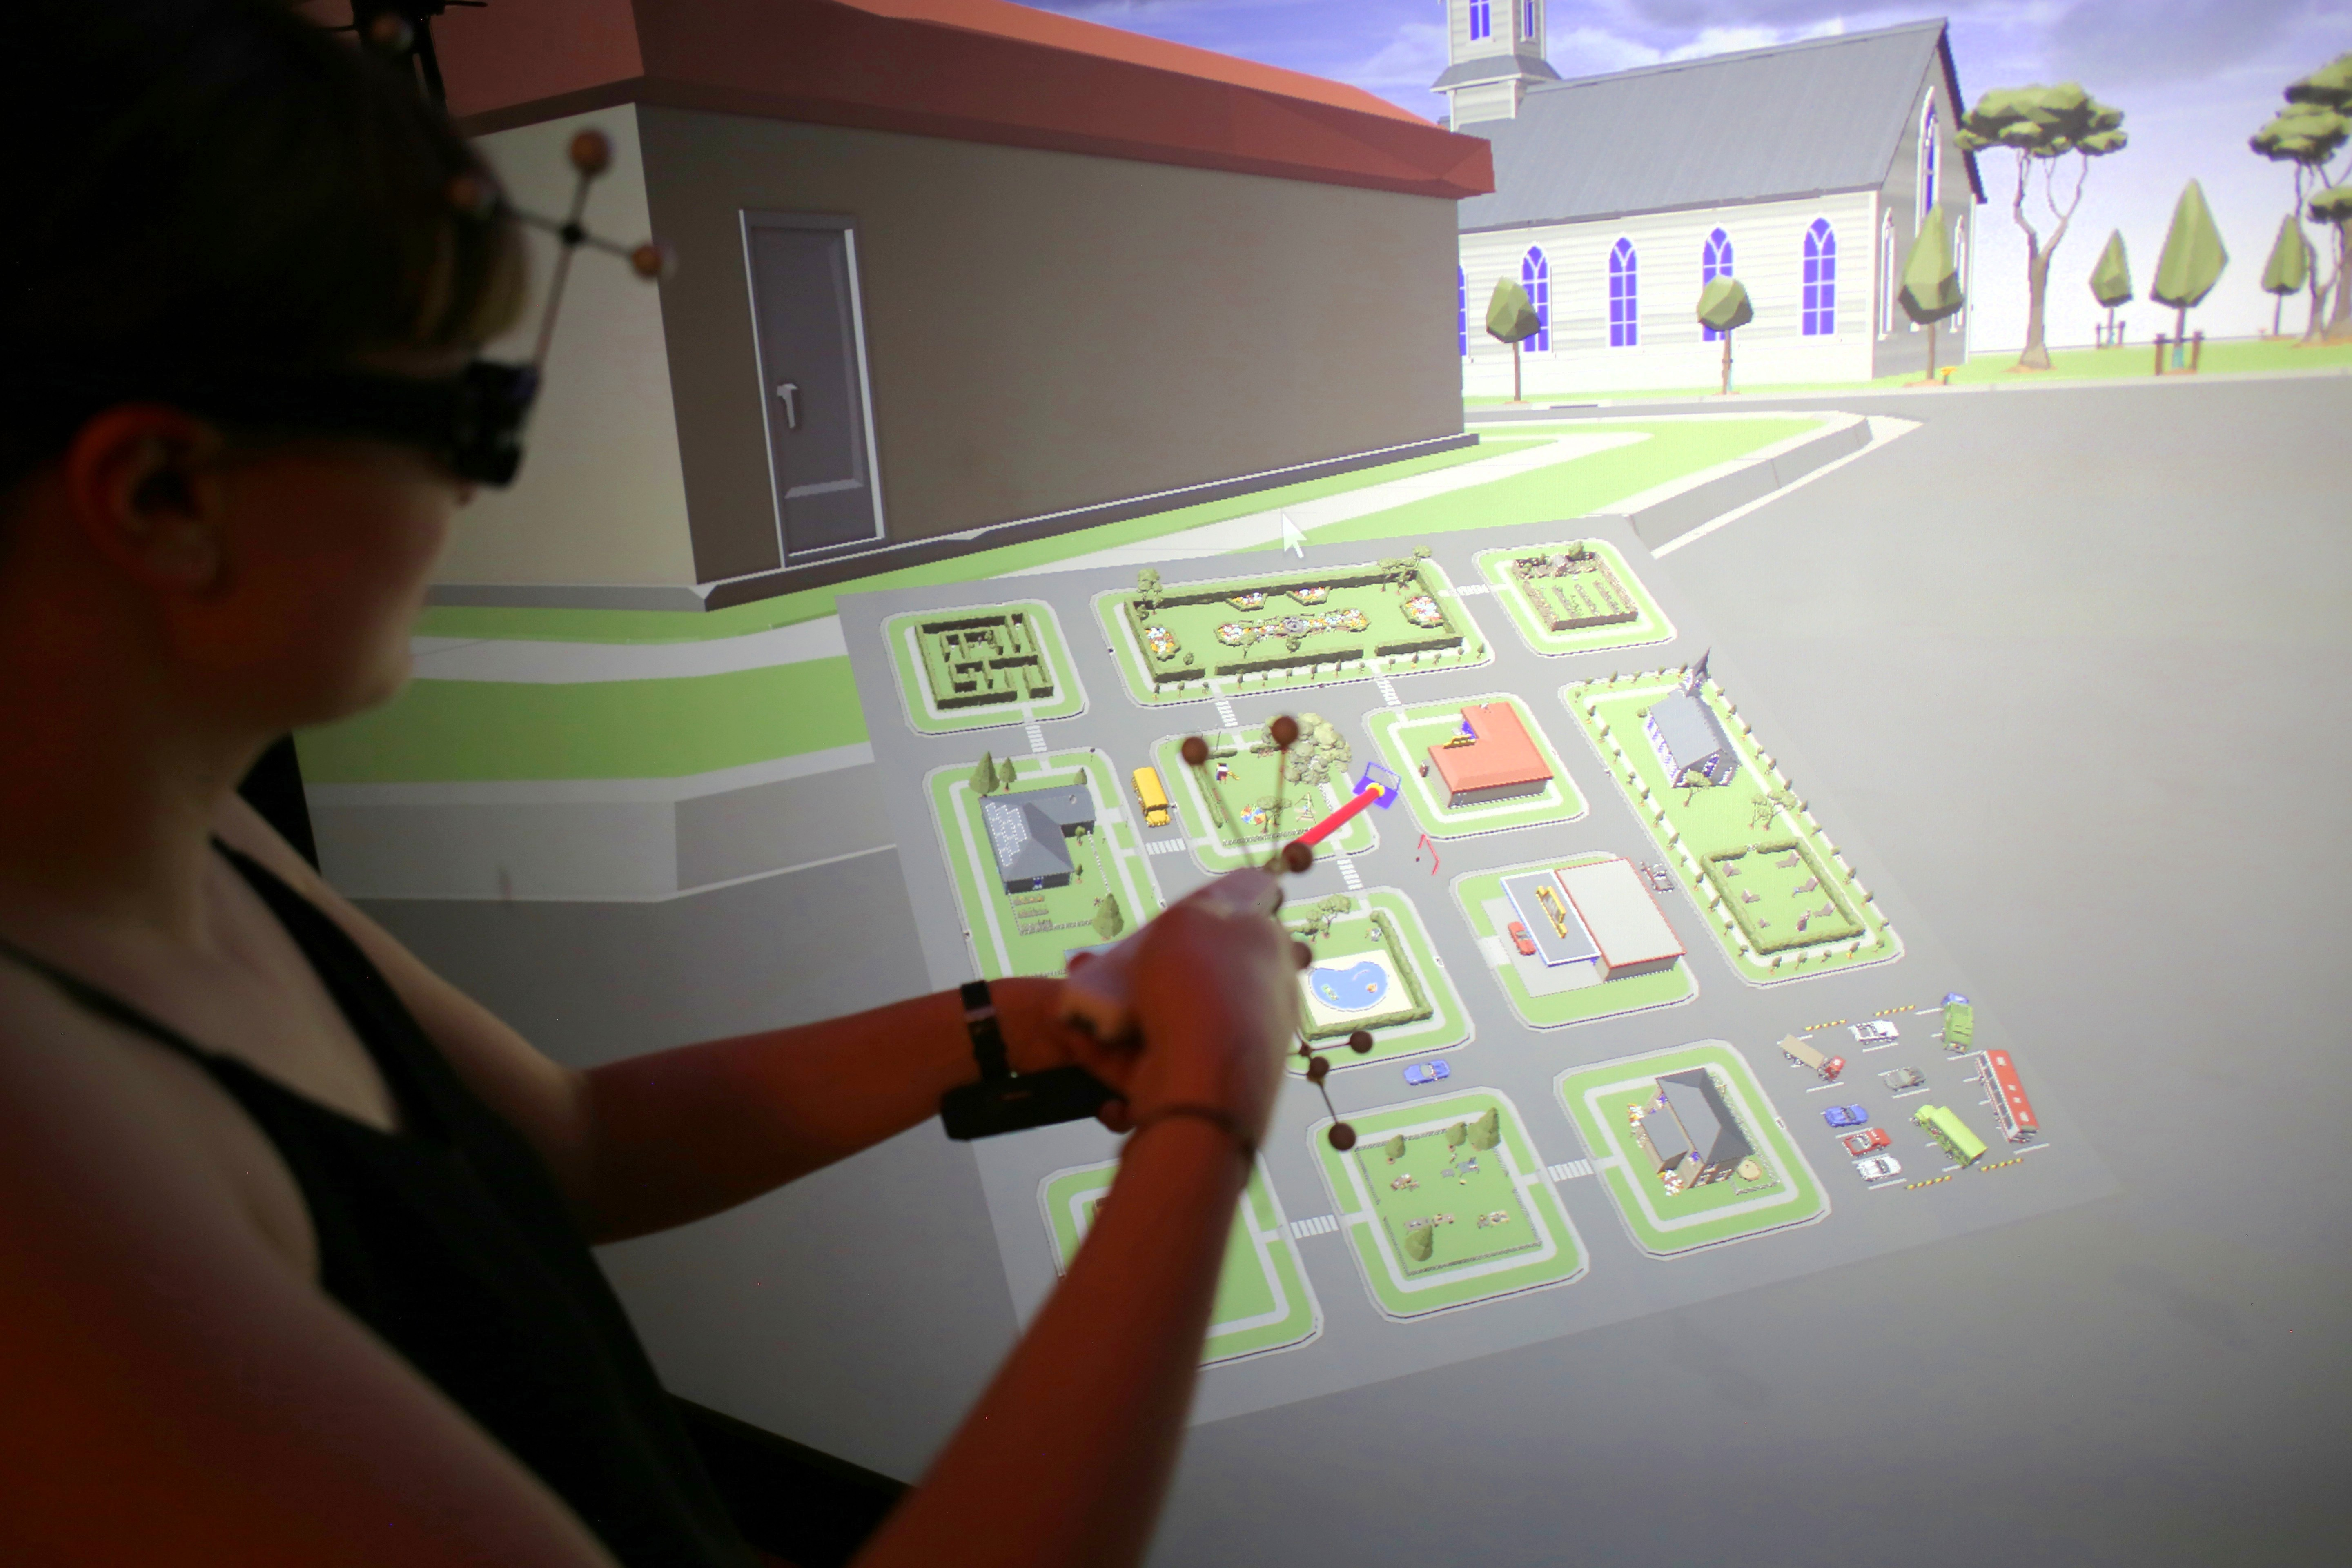
\includegraphics[width=0.8\textwidth]{images/wim_in_hand.JPG}
  \caption{Hält ein Nutzer die WIM in der Hand, so kann er sie sehr intuitiv bedienen. Allerdings könnte er sie für andere verdecken.}
  \label{fig:todo}
\end{figure}

Die erste Herangehensweise war, die WIM an einen getrackten Gegenstand zu koppeln. In diesem Fall bestand dieser aus einem Holzwürfel mit fünf reflektierenden Kügelchen.
Dies ermöglicht verschiedene Szenarien einfach durch zu spielen, indem man den Holzwürfel an verschiedenen Stellen im Raum platziert oder ein Nutzer diesen in die Hand nimmt.

Mit der WIM in der nicht-dominanten Hand kann der Nutzer diese sehr gut drehen und sie somit aus (fast) allen Richtungen einsehen. Dabei kann er mit seiner dominanten Hand die gewünschte Position auswählen. Dieses Zusammenspiel mit der groben Justierung der WIM in der linken und der feingliedrigen Interaktion mit der rechten Hand funktioniert sehr natürlich.
In unserer Testversion wurde die WIM stets unsichtbar gestellt, sobald der Holzwürfel unterhalb der Hüfte gehalten wurde.

Der steuernde Nutzer hält die WIM nämlich oft so, dass die wichtigen Punkte für ihn sichtbar sind, jedoch nicht zwangsläufig für die anderen Nutzer. Dies kann noch verschlimmert werden, wenn die WIM durch den Körper der Person verdeckt wird.


\subsection{Tabletop}
Eine weitere Möglichkeit ist die Platzierung der WIM auf einem Holotisch, wie er in unserem Labor verfügbar ist.
Dadurch wäre die WIM für alle sichtbar und gleichzeitig nicht im Sichtfeld auf die Hauptszene. Gleichzeitig bedeutet dies allerdings, dass bei jedem Navigationsvorgang die Aufmerksamkeit der Nutzer von der Szene zum Tisch wandern muss, was denn Interaktionsfluss stören kann. Diese Option wurde im Rahmen der Arbeit nicht implementiert.

\subsection{Zentral, Mitte der Nutzergruppe}


\begin{figure}[h!]
  \centering
  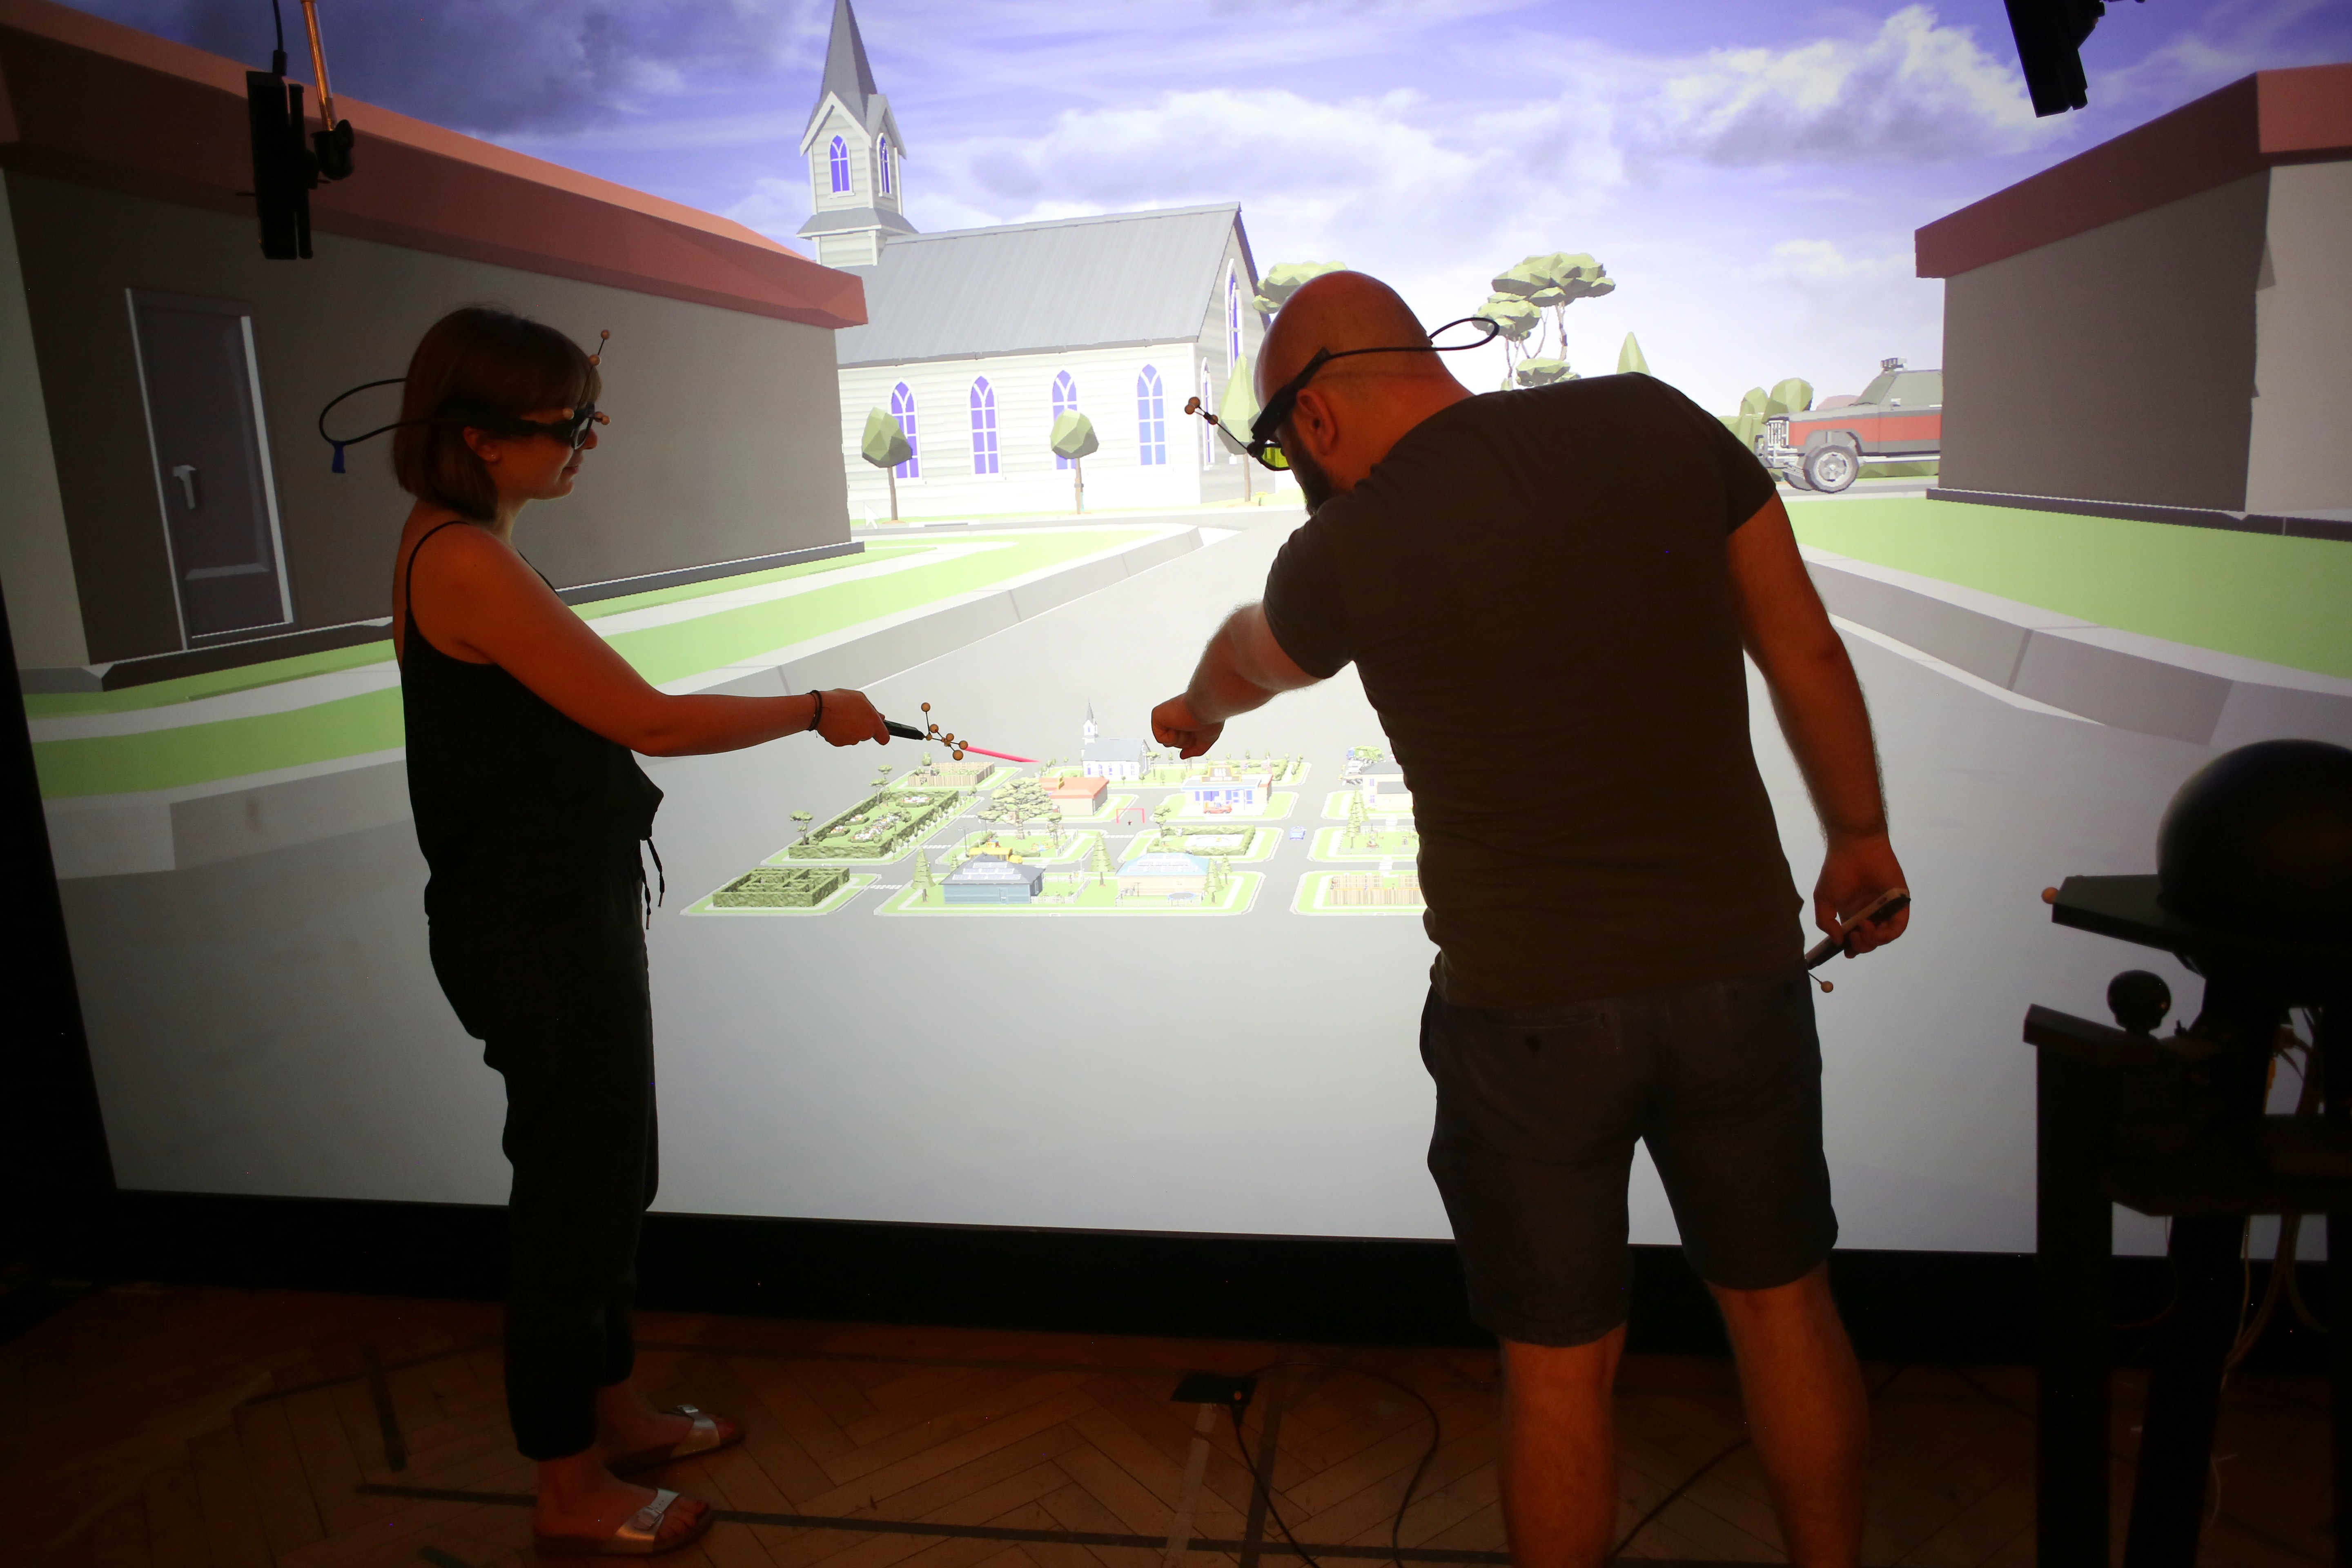
\includegraphics[width=0.8\textwidth]{images/wim_zentral.JPG}
  \caption{Steht die WIM zentral zwischen der Nutzergruppe, ist sie für alle einseh- und bedienbar.}
  \label{fig:todo}
\end{figure}

Stellt man die WIM zentral vor die Nutzergruppe (also kurz vor die Leinwand) bringt dies den Vorteil mit sich, dass sie von allen Nutzern gut eingesehen werden kann.
Dabei ist es von Nöten, dass sie durch eine zusätzliche Eingabe drehbar ist, da man sonst Teile, die nur von der Rückseite der Leinwand aus sichtbar wären, nicht auswählen kann.
In unserem Fall wurde dies durch das Drehen eines Joysticks am Spheron ermöglicht.
Als optimale Höhe stellte sich dabei ungefähr 1,30 Meter heraus. So kann man die WIM gut überblicken und muss sich gleichzeitig nicht zu weit bücken

Angelehnt an Kunert et al. \cite{Kunert2014Photoportals} wurde ebenfalls eine Möglichkeit implementiert, bei der sich die WIM sowohl in der Hand, als auch in zentraler Position befindet. Solange ein Nutzer den Holzwürfel in der Hand hat, befindet sich die WIM ebenfalls dort. Stellt er ihn in der Nähe des Spherons ab, wird die WIM mit diesem gekoppelt und befindet sich ab diesem Moment in der oben beschriebenen Zentralposition.

\subsection{Projektion am Boden}
Wie bereits im vierten Kapitel beschrieben, wäre es ebenfalls denkbar, die WIM mit einer Projektion am Boden darzustellen, wie bei Stoakley et al. \cite{Stoakley2010VirtualWIM}.
Damit hätte man den Vorteil, dass die WIM direkt bedient werden könnte und gleichzeitig nicht im Weg ist. Grundsätzlich kann die WIM dabei zwei- und dreidimensional sein (wobei letzteres für Mehrbenutzer einen extremen Mehraufwand auf Hardwareseite mit sich bringen würde). Diese Variante wurde im Zuge dieser Arbeit wegen des hohen technischen Aufwandes nicht implementiert.

\section{Größe der WIM}
Die quadratische Testumgebung hat eine Seitenlänge von 125 Metern, wobei nur der zu bereisende Bereich eine Größe von etwa 100 Metern aufweist.
Der Maßstab wird dabei 1:100 gewählt. Mit dieser Größe können alle Teile der WIM gut erreicht werden und die miniaturisierte Plattform ist mit einer Breite von 5 cm gut erkennbar. 
Dennoch wird den Nutzern die Möglichkeit gegeben, die Skalierung der WIM zu ändern. Dies wird erreicht, indem der Nutzer mit gedrückten Skalierungsknopf seinen Pointer vom Zentrum der WIM weg oder auf dieses zu bewegt. Dabei wird die Skalierung entsprechend des Verhältnisses von der aktuellen Distanz zum Zentrum und der Ausgangsdistanz gewählt (Beispiel: Der Nutzer drückt in einer Distanz von einem Meter von Zentrum den Knopf und verringert die Distanz auf 50 Zentimeter. Die WIM wird folglich um die Hälfte herunterskaliert).

Die Größe der WIM hat eine wichtige Auswirkung auf die Bedienbarkeit der Technik und somit auch der Bearbeitungszeit der Technik. Im folgenden Kapitel (9.1.1) wird darauf näher eingegangen.

\section{Platzierung der Nutzerplattform}
Um das Ziel der Reise zu bestimmen soll die Plattform so platziert werden können, dass jede mögliche und gewünschte Position und Orientierung erreichbar ist., wobei der Aufwand der Platzierung minimal gehalten werden soll.

\subsection{Positionierung in der Luft}

\begin{figure}[h!]
  \centering
  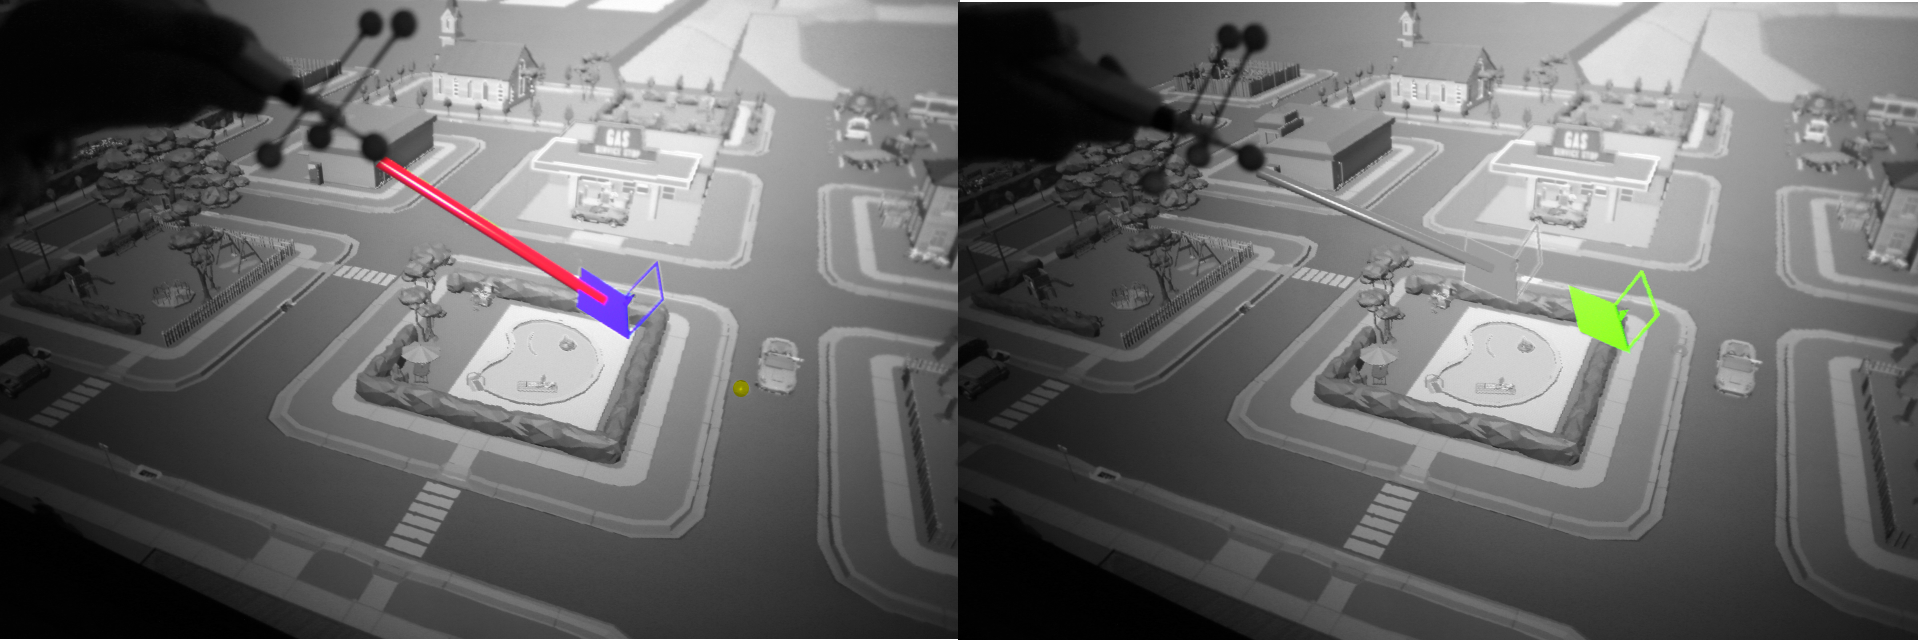
\includegraphics[width=0.8\textwidth]{images/fork.png}
  \caption{Mit der Gabeltechnik ist es möglich die Plattform in der Luft zu positionieren. Dabei visualisiert der gelbe Punkt die Blickrichtung. Auf Knopfdruck wird diese Position bestätigt und die grüne Plattform zeigt die Position nach dem Teleport.}
  \label{fig:todo}
\end{figure}


Um die Plattform in der WIM zu platzieren, sodass sie schwebend mit freier Rotation im Raum steht, wurde eine Art \textit{Gabel-Technik} entwickelt. Hierbei wird an das Ende des Pointers ein kurzer (ca. 20cm) Strahl gehängt, an dessen Ende sich die Miniatur befindet (in der Abbildung in blau zu sehen). Wird die aktuelle Position dieser Repräsentation in der WIM durch einen Klick bestätigt, wird eine Kopie erstellt, die die finale Position widerspiegelt, die die Nutzer nach der Reise haben werden (siehe in Grün in der Abbildung).
Somit ist es den Nutzern möglich ihre Orientierung und Position in der Welt frei zu bestimmen, um z.B. auch von oben auf Gebäude blicken zu können.


\subsection{Positionierung am Boden}
Will die Nutzergruppe entlang des Bodens ausgerichtet bleiben, bieten wir folgende Möglichkeiten:

\subsubsection{Direkte Auswahl}

\begin{figure}[h]
  \centering
  \includegraphics[width=0.8\textwidth]{images/direct.png}
  \caption{Direkte Auswahl: Für die schnelle und effiziente Auswahl wird die Plattform, sobald man den Boden schneidet, entlang der Strahlrichtung ausgerichtet.}
  \label{fig:todo}
\end{figure}

Berührt die blaue Plattform der \textit{Gabel-Technik} den Boden, so wird sie automatisch entlang diesem ausgerichtet. Die Sichtrichtung der Gruppe ist dabei immer entlang der, in die Bodenebene projizierten, Strahlrichtung vom Pointer weg. Dadurch wird eine sehr direkte Form der Positions- und Richtungsauswahl ermöglicht, die man mit einem kurzen Knopfdruck bestätigen kann. Auch in diesem Fall wird eine grüne Kopie der vormals blauen Plattform erstellt.

\subsubsection{Position und Blickrichtung}

\begin{figure}[h]
  \centering
  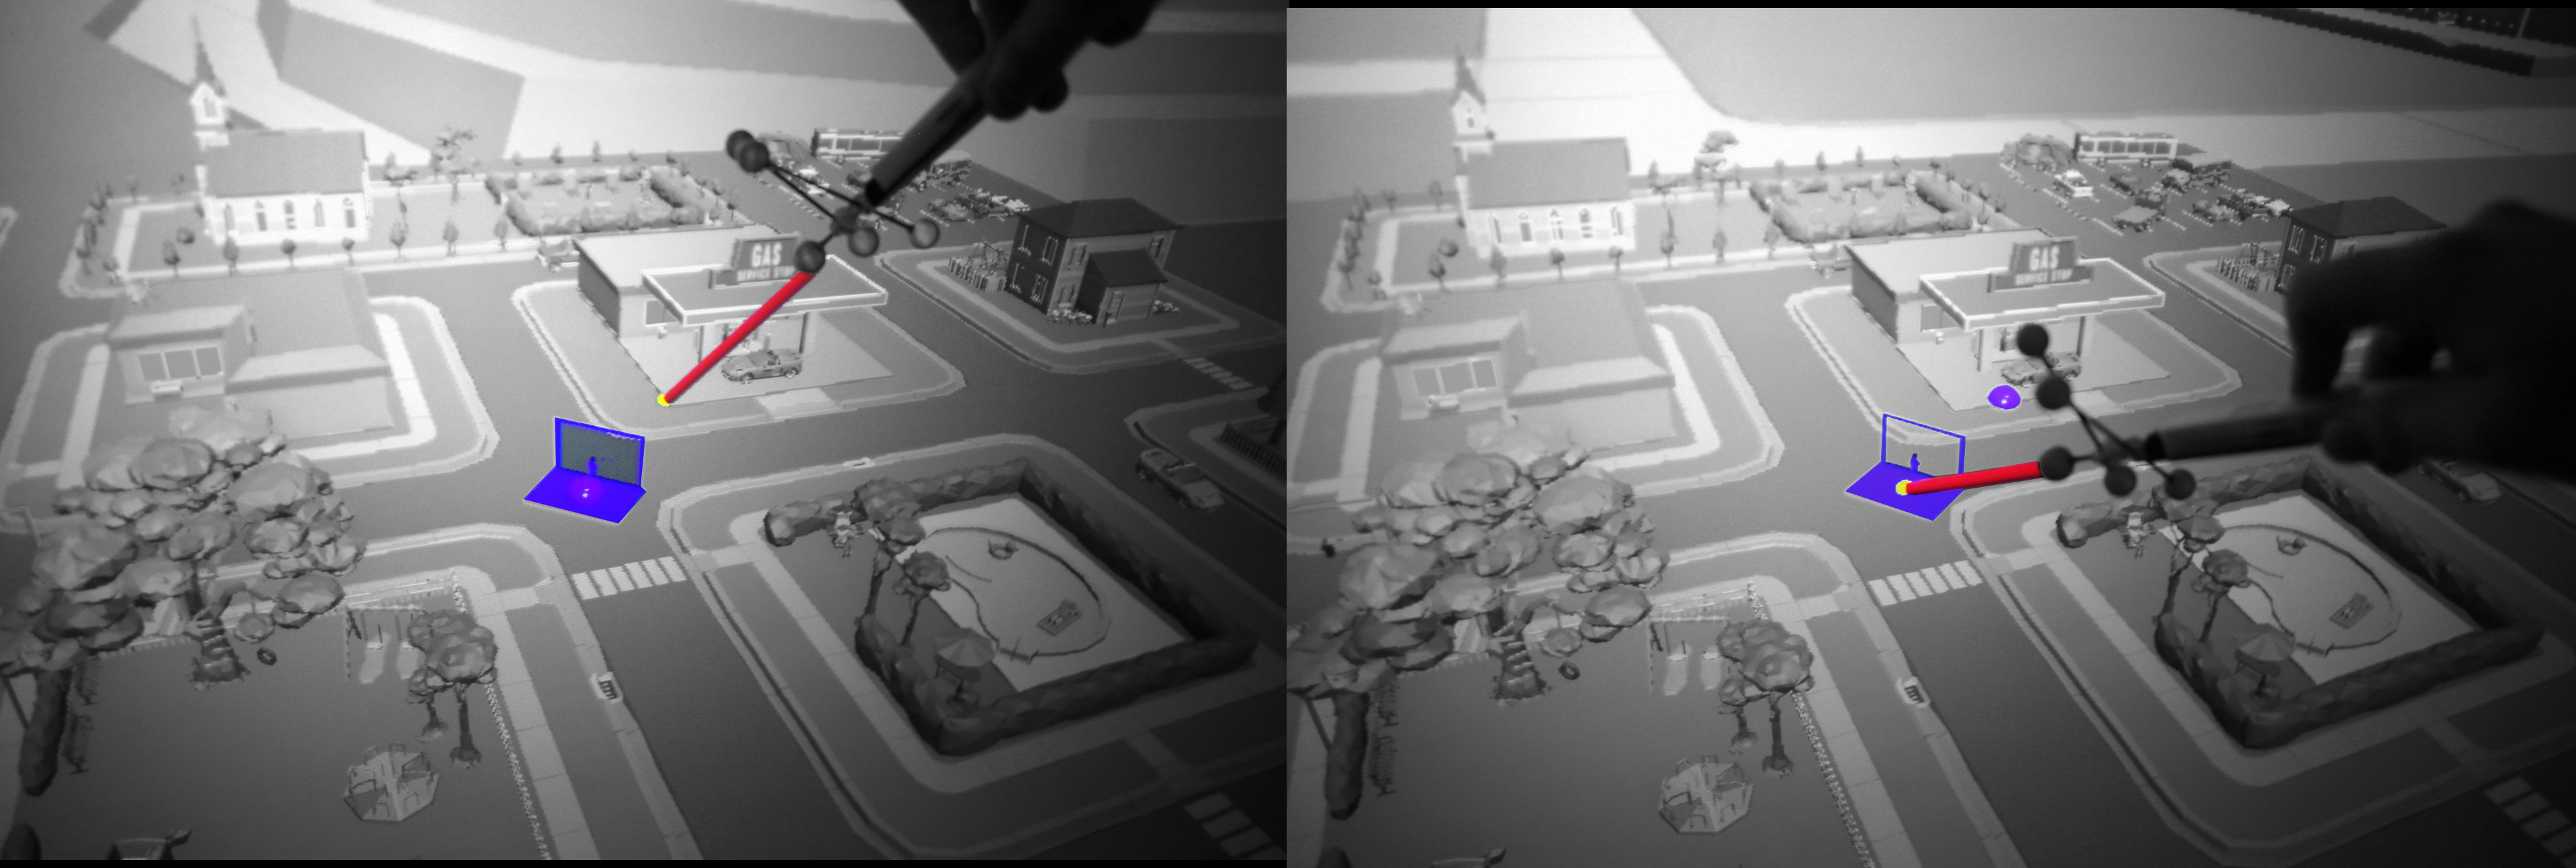
\includegraphics[width=0.8\textwidth]{images/look.jpg}
  \caption{Position und Blickrichtung: Hält man den Knopf länger gedrückt, während man den Boden schneidet bietet das System zwei Möglichkeiten: Entweder die Plattform wird an den aktuellen Punkt gesetzt und man bestimmt fortan die Blickrichtung (links) oder man wählt erst den Punkt den man sehen will und positioniert danach die Plattform, die dann immer in Richtung dieses Punktes ausgerichtet ist (rechts)}
  \label{fig:todo}
\end{figure}


Hält man den Knopf allerdings länger gedrückt, so bestätigt man, dass der aktuelle Schnittpunkt mit der WIM der Punkt ist, den man gerne sehen möchte. Hält man den Knopf nun weiterhin gedrückt, kann man die Position der Plattform wählen, wobei diese immer in Richtung des Anfangs gewählten POI ausgerichtet ist.
Natürlich ist es auch möglich, eine umgekehrte Version dieser Technik zur Verfügung zu stellen. In diesem Fall wird durch langes Drücken erst die Position der Plattform gewählt, welche dann in Richtung des aktuellen Schnittpunkts mit der WIM ausgerichtet wird. 
Generell lässt sich aber sagen, dass die erste Methode in den meisten Fällen als etwas besser bedienbar eingeschätzt wurde, da man damit sicherstellen kann, dass wirklich alle Bestandteile des POI`s innerhalb des sichtbaren Bereichs sind.

\subsection{Plane of Interest}

Zusätzlich zu den Platzierungstechniken, die bisher beschrieben wurden, gibt es weiterhin die Möglichkeit, sogenannte \textit{Planes of Interest} zu erstellen. Diese sind ebenfalls Kopien der Nutzerplattformen, welche frei in der WIM positioniert werden können. Die Platzierung funktioniert dabei kontextabhängig:
Zeigt der Nutzer in die WIM, so läuft sie analog zu den in den vorherigen Unterpunkten beschriebenen Vorgängen ab, wobei durch den Klick eines anderen Knopfes (\textit{PLOI-Knopf}) keine grüne, sondern eine weiße Plattform erscheint. Schneidet man zukünftig diese mit dem Selektionsstrahl, so erhält die blaue Plattform die Ausrichtung und Position der weißen.

\begin{figure}[h!]
  \centering
  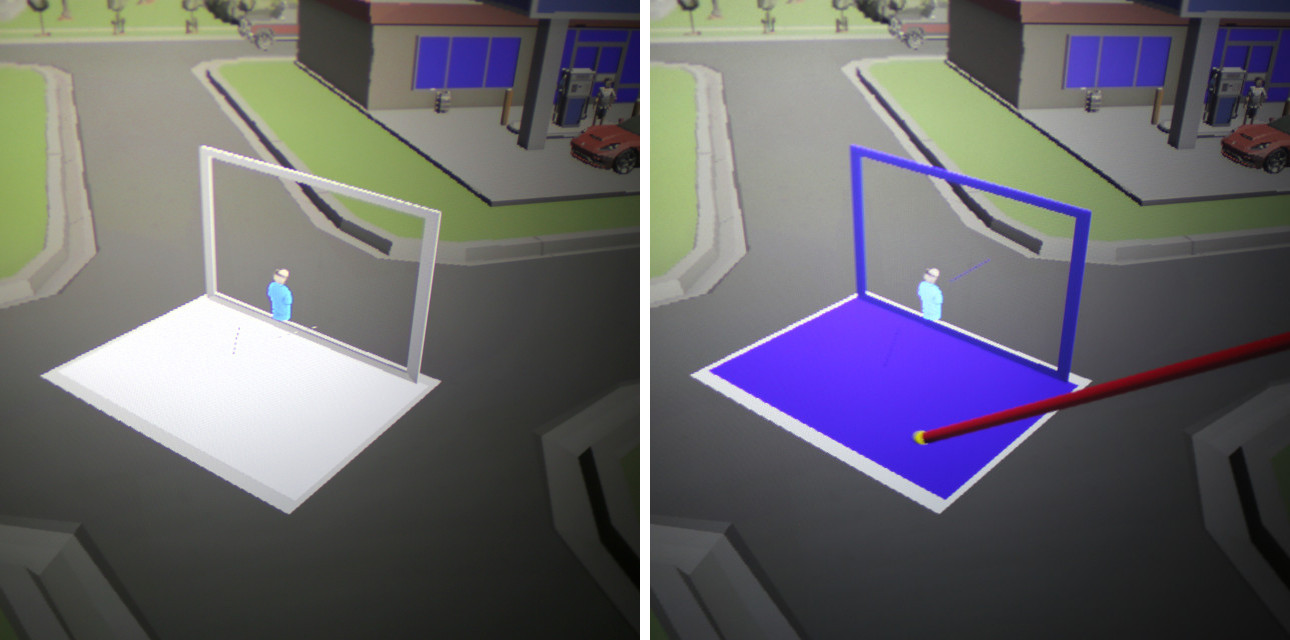
\includegraphics[width=0.8\textwidth]{images/platform_bluewhite.JPG}
  \caption{Mit der sogenannten \glqq Plane of Interest\grqq{}, lassen sich Aufenthaltsorte speichern. Schneidet man diese weißen Plattformen mit dem Selektionsstrahl so wird die blaue Plattform direkt entsprechend der weißen ausgerichtet.}
  \label{fig:todo}
\end{figure}

Dadurch lassen sich für später oder für andere Nutzer Orte speichern, die dann ohne großen Aufwand angesteuert werden können.
Zeigt der Nutzer allerdings nicht in die WIM, so wird auf Knopfdruck der aktuelle Aufenthaltsort gespeichert, indem ebenfalls eine weiße Plattformkopie erstellt wird. So kann der aktuelle Ort zu späteren Zeitpunkten gespeichert werden.
Will man eine \textit{Plane of Interest} wieder löschen, so drückt man erneut den \textit{PLOI-Knopf}, während man die entsprechende \textit{Plane of Interest} schneidet.


\section{Platzierung des Portalfensters}
Hat man nun die grüne, finale Preview in der WIM platziert, soll der Teleport, wie bereits beschrieben, durch Vergrößerung eines Portalfensters geschehen, welches einen Vorabblick in die neue Szene bietet. Dabei stellt sich die Frage, wo und zu welchem Zeitpunkt dieses Fenster sichtbar sein soll.

\begin{figure}[h!]
  \centering
  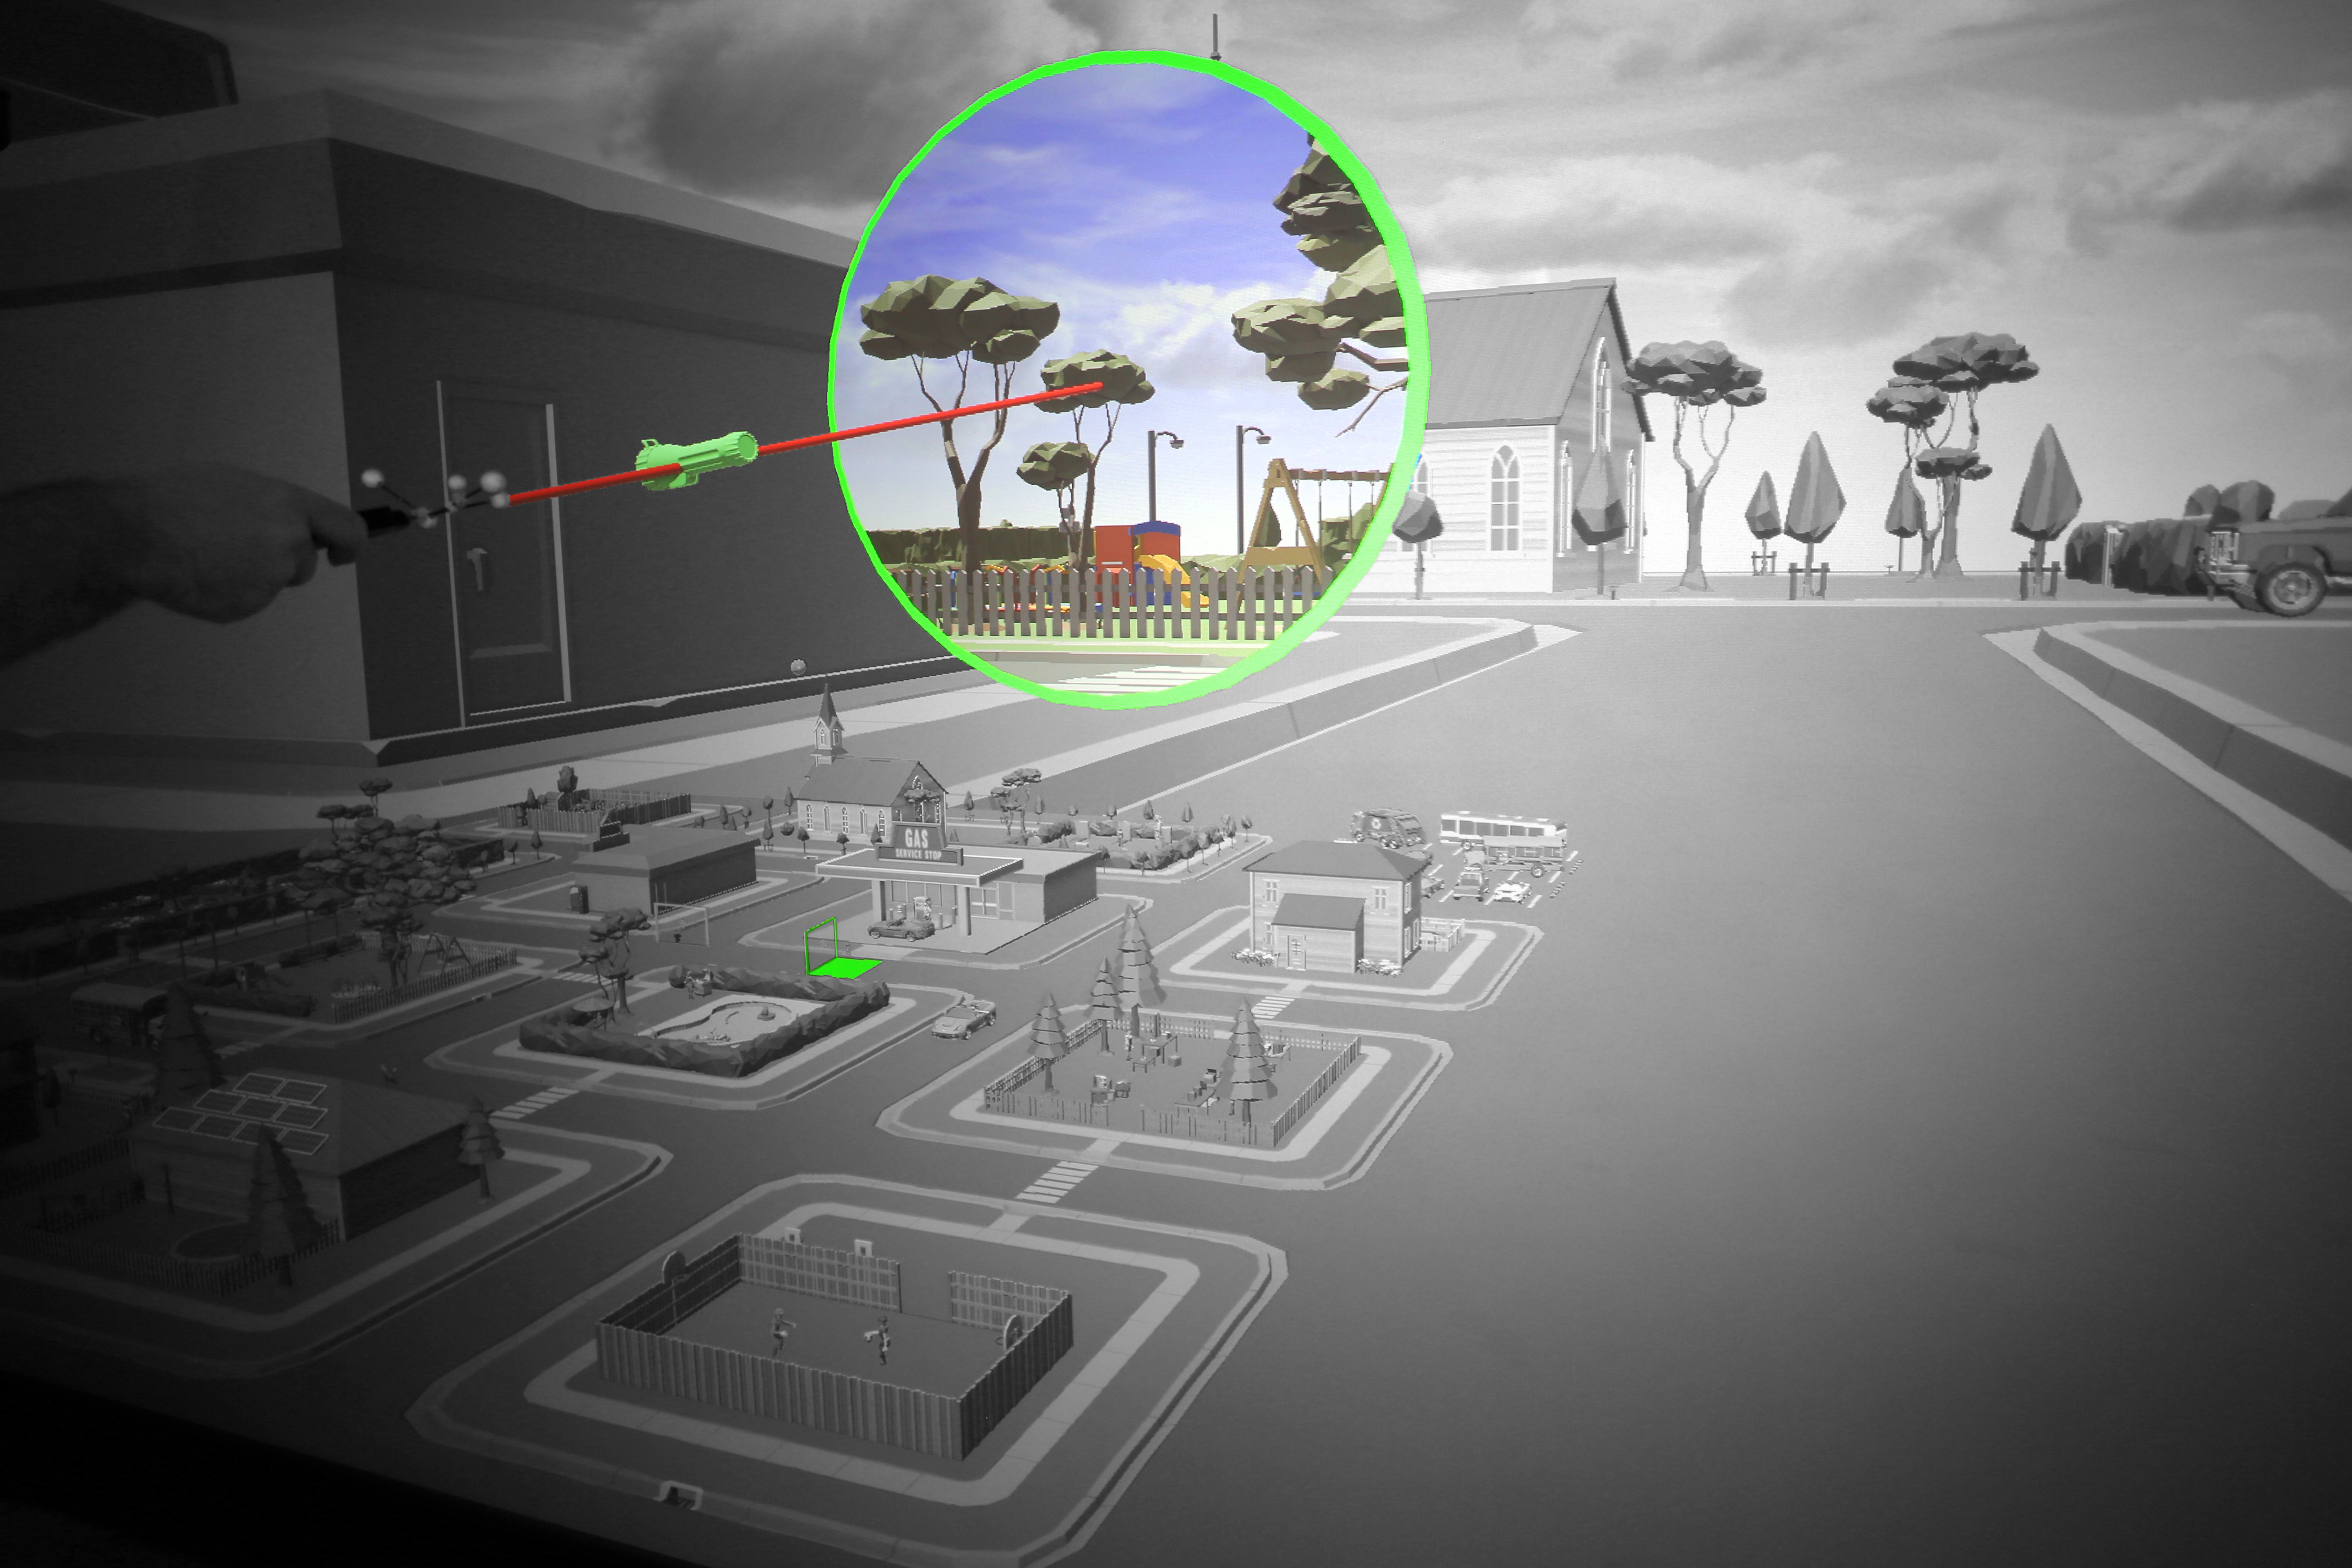
\includegraphics[width=0.8\textwidth]{images/peephole.jpg}
  \caption{Sobald die geplante Position bestätigt wurde erscheint über der grünen Plattform eine Taschenlampe. Greift man diese, erstellt man damit ein Guckloch, welches den Blick auf den Ort nach dem Teleport zeigt.}
  \label{fig:todo}
\end{figure}

Eine Möglichkeit wäre, dass das (in diesem Fall kugelförmige) Portal nach der Zielbestätigung direkt über der WIM bzw. dem gewählten Punkt erscheint. In diesem Fall wäre der Einstieg durch ein Aufblähen der Kugel denkbar.
Auch vorstellbar wäre, wie bei \cite{Kunert2014Photoportals}, das (in diesem Fall zwei- oder dreidimensionale) Fenster an eine Portalkamera oder seinen Pointer zu binden, sodass ein Nutzer, indem er seinen Kopf hineinsteckt, die neue Perspektive vor dem eigentlichen Teleport erkunden kann. Hierbei stellt sich aber der Einstieg problematisch dar: Es ist gut möglich, dass das Fenster von anderen Nutzern kaum oder nicht gesehen wird und eine Transition unvermittelt kommen kann.
Dies gestaltet sich einfacher, wenn das (in diesem Fall eher zweidimensionale) Fenster mittig, zentral und für alle sichtbar auf der Leinwand platziert wird (vgl. Galerie-Modus \cite{Kunert2014Photoportals}). So können  alle Nutzer das Fenster sehen und sind auf den Teleport, welcher durch Vergrößerung des Lochs stattfindet, vorbereitet.
Vor allem in diesem Fall stellt sich aber die Frage, ob dieses Portal sofort nach dem Platzieren der Miniaturplattform erscheinen soll. Es ist nämlich möglich, dass das Portal anderen Nutzern, die ggf. in diesem Moment die Umgebung erkunden die Sicht auf Dinge verdeckt. In einem solchen Fall sollte das Portal nicht sofort Erscheinen und im Zweifelsfall von jedem Nutzer wieder entfernt werden können.

Als Lösung für diese Problematik wurde die Funktion des Strahlwerkzeugs erweitert, damit ein solches \glqq Guckloch\grqq{} erzeugt und bewegt werden kann.
Zeigt der Nutzer mit seinem (ins unendlich verlängerten) Strahl in die WIM, so stehen ihm die oben aufgezählten Platzierungswerkzeuge zur Verfügung. Platziert er nun die (grüne) Plattform in der WIM so erscheint über dieser eine Taschenlampe, welche gegriffen werden kann. Richtet man diese Taschenlampe nun gegen die Leinwand, erscheint das Portal, wobei wie bei einem Taschenlampenkegel der Durchmesser dieses Lochs durch die Distanz der Taschenlampe zur Leinwand bestimmt wird. Will nun ein anderer Nutzer dieses Loch wieder aus seinem Sichtfeld entfernen, kann er mit seinem Strahl auf dieses zeigen, wobei dieser automatisch verlängert wird, wenn der Nutzer nicht mehr in die WIM zeigt. Dabei verschwindet die blaue Plattform vom Ende des Strahls. Der Nutzer kann dieses Loch nun selektieren und, während er den Button gedrückt hält, dieses an eine andere Stelle bewegen bzw. einfach außerhalb der Leinwand ziehen, woraufhin dieses verschwindet.
Klickt einer der Nutzer kurz auf das Loch so öffnet sich dieses wie beschrieben.

\section{Skalierung nach Teleport}
Im Rahmen der Technik ist es grundsätzlich möglich, die Skalierung der Nutzer in der Welt zu vergrößern bzw. zu verkleinern. Dies ermöglicht, dass Nutzer auch kleine Merkmale der Umgebung bis im Detail erkunden können oder durch Aufskalierung die Umgebung besser überblicken können. Dabei stellt sich die Frage, ob die aktuell gewählte Skalierung nach dem Teleport beibehalten werden soll oder ob man nach jedem Sprung wieder auf die Ausgangsgröße zurückskaliert wird. Beide Vorgehensweisen sind je nach Aufgabe und Motivation legitim. Für das Beispiel der virtuellen Stadtführung sind zum Beispiel beide Ausführungen denkbar. Entweder will der Stadführer, nachdem die Gruppe auf die Größe mehrerer hundert Meter vergrößert wurde, um eine schöne Aussicht über die Dächer der Stadt zu erhalten, diese nach dem Teleport beibehalten oder beim Besuch der nächsten Stadt wieder - in Menschengröße - zwischen den Straßenschluchten stehen.

\section{Steering Navigation}

\begin{figure}[h!]
  \centering
  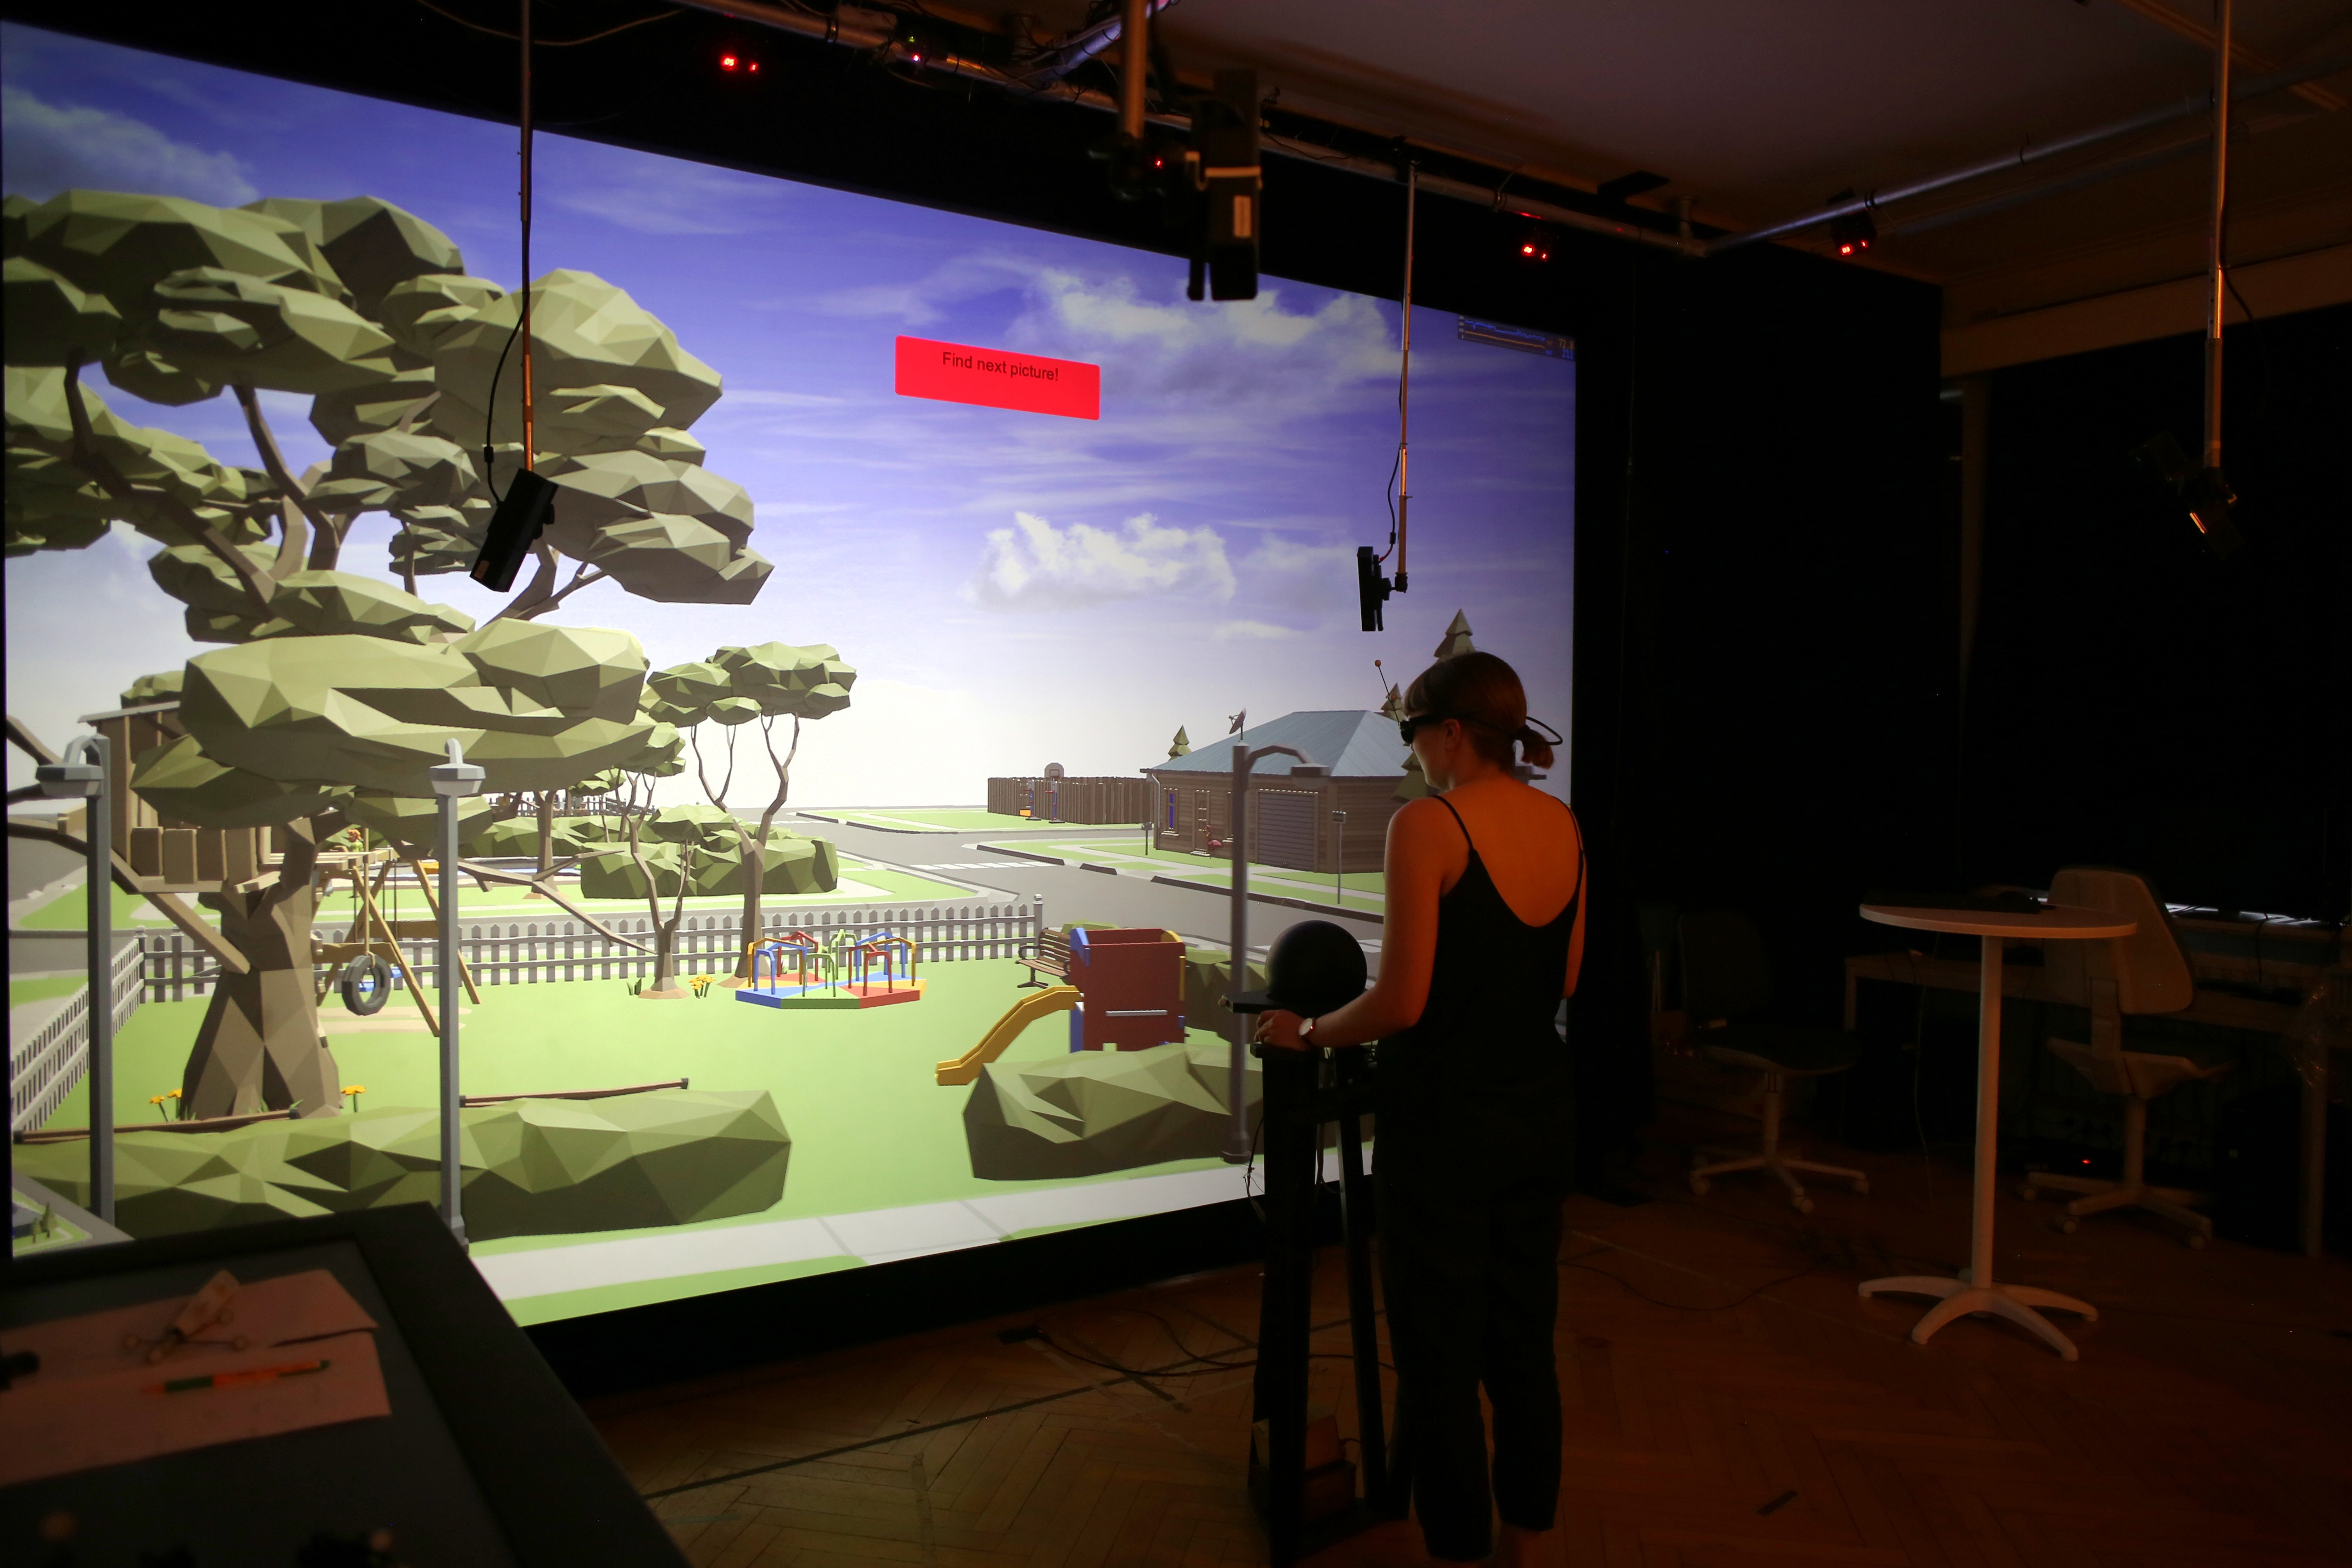
\includegraphics[width=0.8\textwidth]{images/steering.jpg}
  \caption{Zum Nachjustieren bietet das System Steering Navigation.}
  \label{fig:todo}
\end{figure}


Obwohl im besten Falle die Teleportationstechnik ausreicht, um ein Ziel zu erreichen, wird zusätzlich eine Möglichkeit zur Steering-Navigation angeboten. Dabei dient ein Spheron als 6-DOF Eingabegerät (vgl. \cite{Kulik2011C1x6}), mit dem man sich über kurze Distanzen (z.B. zum Nachjustieren nach dem Teleport) navigieren kann.

\section{Finales Interaktionsdesign}
Zur Durchführung einer Studie (mit jeweils zwei Nutzern) wurde folgendes Interaktionsdesign umgesetzt:
Um eine möglichst einfache und für alle sichtbare Interaktion mit der WIM zu ermöglichen, wurde die WIM auf eine feste Höhe von 1.30 Metern kurz vor der Leinwand platziert. Das Entkoppeln, sodass man sie in der Hand halten kann, wurde deaktiviert, da dies einerseits durch zahlreiche Drehungen die Raumwahrnehmung verschlechtern kann, andererseits sollten die Interaktionsmöglichkeiten nicht zu umfangreich sein, um unerfahrene Nutzer nicht zu überfordern. Die anfängliche Größe der WIM liegt bei 1.20 Metern, wobei die Nutzer diese wie oben beschrieben ändern können.
Die WIM ist mit Hilfe einer \textit{Spacemouse} drehbar, jedoch wird die WIM bei jedem öffnen und nach jedem Teleport wieder mit Norden nach oben ausgerichtet.
Dies soll dazu beitragen, dass Nutzer sich ein besseres räumliches Verständnis aneignen können (vgl. Kapitel 5).
Jeder der Nutzer besitzt ein Werkzeug, mit dem er die Technik bedienen kann. 
Für die Platzierung am Boden wird (neben der "Direkten Auswahl" (s.o.)) nur die Methode genutzt wird, erst den POI auszuwählen, dann Plattform in Blickrichtung dessen zu positionieren. Auch hier war der Grund, dass die Nutzer nicht mit zu vielen Möglichkeiten konfontiert werden sollen und diese Methode in Vortest als angenehmer eingeschätzt wurde.
Auch die Möglichkeit Planes of Interest zu platzieren wurde im Zuge dessen deaktiviert. Es kann immer nur eine Instanz der grünen finalen Plattform geben, aus der immer nur eine Portal erzeugt werden kann.
Bei jedem neuen Setzen verschwindet das Portalfenster.
Da in unserem beispielhaften Studiendesign ausschließlich Ziele am Boden bereist werden, wird statt der WIM eine unsichtbare Bodenplatte geschnitten, damit nicht durch Fehleingaben aus Versehen die Plattform auf Dächern oder Hecken gesetzt wird.
Bis auf die Skalierung der WIM werden alle Interaktionen durch die Verwendung eines einzigen Knopfes durchgeführt.
Die Skalierung der Nutzergruppe wird in der Studie nicht verändert, da alle zu bereisenden Ziele in der Skalierung eins zu eins aufzusuchen sind.
Zusätzlich zur Teleportationstechnik steht den Nutzern der Spheron zum Nachjustieren nach dem Teleport zur Verfügung. Grundsätzlich ist es aber aufgrund der vorher festgelegten Ziele nicht notwendig diesen auch zu nutzen, da alle Ziele mit der Teleportationstechnik alleine gefunden werden können.